\section{Promises}

Das Prinzip der asynchronen Verarbeitung, bringt Komplexität nach sich. Um dem entgegenzuwirken, hat man in dieser Arbeit schon das Prinzip der Callbacks kennengelernt. Dank der Rückruffunktionen ist es Möglich auf blockierende Aktionen zu warten bis diese eingetroffen sind. Sollten jedoch mehrere asynchrone Events voneinander Abhängig sein, kann das schnell zu unübersichtlichem Code führen (siehe Abb. \ref{Nested-Callback-with-catch-error}). Mit Promises können voneinander abhängige Operationen übersichtlich dargestellt werden.\\

\noindent
Ein Promise repräsentiert ein Objekt das noch nicht absehbar ist, aber in Zukunft genutzt werden soll. Als Beispiel könnte man den Inhalt einer Datei, die von einem File-Server in einem Browser geladen werden soll, nehmen. Dieser ist auf Anhieb nicht verfügbar, da die Daten zunächst über das Netzwerk übertragen werden müssen. Anstatt auf den Download zu warten, führt der Browser diesen Prozess asynchron aus. Wenn die Daten angekommen sind, führt das Promise-Objekt die Aktionen mit den erstellten Verarbeitungsmethoden fort. Dank der Promise-Verkettung ist es auch möglich Fehlerbehandlungen übersichtlich abzudecken. Während bei Callbacks das Ergebnis der Interaktion sofort verarbeitet werden muss, basieren Promises nach ihrem Verarbeitungsstatus. Das heißt sie können mit dem Ergebnis auch \glqq{}später\grqq{} interagieren.

\subsection{Funktionsweise}

\noindent
Promises \textit{(Versprechen)} verhalten sich in Javascript ähnlich wie im echten Leben. Die Definition aus dem Wörterbuch ist: Das Versprechen ist eine einseitige Zusage über eine zukünftige Handlung oder ein zukünftiges Ereignis\cite{versprechen}.\\

\noindent
Das heißt:

\begin{description}
    \item Ein Versprechen ist eine Absicherung, dass etwas gemacht wird. Unabhängig davon, ob das Versprechen sich selbst oder von einer anderen Partei gegeben wird.
    
    \item Ein Versprechen kann eingehalten oder gebrochen werden.
    
    \item Wurde ein Versprechen nicht eingehalten, möchte man den Grund für die Nichteinhaltung wissen, um darauffolgend zu handeln.
    
    \item Beim Zeitpunkt eines Versprechens hat man nur die Absicherung. Man kann damit erstmal noch nichts anfangen. Es kann nur geplant werden was nach dem Einhalten des Versprechens gemacht wird. Dementsprechend kann man auch Maßnahmen setzen beim Nichteinhalten dieser Absicherung.
    
\end{description}

\noindent
Es gibt zwei grundlegende Prinzipien der Promises, die zu Verstehen sind: Das \textbf{Erstellen von Promises} und das \textbf{Verarbeiten von Promises}.

\subsubsection{Erstellen eines Promises}

\begin{figure}[H]
\begin{lstlisting}[basicstyle=\small]
new Promise( /* executor */ (resolve, reject) => { ... } );
\end{lstlisting}
\caption{Erzeugung einer neuen Promise-Instanz.}
\end{figure}

Der Konstruktor nimmt eine Rückruffunktion als Eingangsparameter. Diese Funktion wird auch \textbf{Executor} genannt\cite{promise-executor}. Der Executor akzeptiert zwei Parameter \textbf{resolve} und \textbf{reject}. Innerhalb dieser Funktion wird eine asynchron blockierende Operation initiiert (z.B. Das suchen einer Datei, eine Datenbankabfrage etc.). Wurde diese asynchrone Operation erfolgreich ausgeführt, ruft der Promise-Konstruktor die resolve Funktion mit dem entsprechendem Ergebnis auf. Anders wird bei einem Fehler die reject Funktion mit der jeweiligen Fehlernachricht aufgerufen.

\begin{figure}[H]
\begin{lstlisting}[basicstyle=\small]
module.exports = {
    mode: 'development',
    entry: './src/modules/promises/introduction.ts',
    ...
}
\end{lstlisting}
\caption{Vor dem Ausführen der Beispiele sollte ../promises/introduction.ts als Eingangsdatei in der webpack.config.js definiert werden.}
\end{figure}

\noindent
Da man nun weiß wie ein Promise erstellt wird, kann auf die unterschiedlichen Vorgehensweisen von Callbacks und Promises eingegangen werden. Die Nutzung von Promises und Callbacks differenzieren sich hauptsächlich im Design und in der Verarbeitung.

\begin{figure}[H]
\begin{lstlisting}[basicstyle=\small]
/*** Callback **/
function getA(callback) {
    return setTimeout(() => callback('a'), 100);
}

function getB(callback) {
    return setTimeout(() => callback('b'), 200);
}

function getC(callback) {
    return setTimeout(() => callback('c'), 300);
}

getA(a =>
    getB(b =>
        getC(c => console.log(a + b + c))
    )
);
\end{lstlisting}
\caption{Darstellung mit Callbacks.}
\end{figure}

\noindent
Die Funktionen werden \textbf{ineinandergeschachtelt}. Die Rückgabewerte befinden sich alle innerhalb des Geltungsbereiches von Funktion getA().

\begin{figure}[H]
\begin{lstlisting}[basicstyle=\small]
/*** Promises **/
function getA(): Promise<string>  {
    return new Promise(resolve =>
        setTimeout(() => resolve('a'), 100));
}
...

getA()
    .then((a: string) => getB().then(b => a + b))
    .then((ab: string) => getC().then(c => ab + c))
    .then((result: string) => console.log(result));
\end{lstlisting}
\caption{Darstellung mit Promises.}
\end{figure}

\noindent
Die Funktionen werden \textbf{aneinandergeschachtelt}. Die Rückgabewerte müssen innerhalb der Kette weitergereicht werden. Hier wird bereits ein kleiner Einblick gewährt, wie man Promises verarbeitet. Promises haben einen Status und einen Wert. Das Promise Objekt, welches getA() zurückgibt, ist beim Aufruf im ausstehenden (pending) Zustand und der Wert ist undefined. Gibt die Funktion setTimeout() den Wert nach der Zeitverzögerung zurück, werden Status und Wert des Promise aktualisiert. Hierbei spricht man vom \textbf{auflösen} eines Promise. Trifft somit der Wert 'a' ein wechselt der Status in den eingetroffenen (resolved) Zustand.

\begin{figure}[H]
\begin{lstlisting}[basicstyle=\small]
export interface FakeHttpResponse {
    code: string;
    message: string;
}

const rejectedPromise = new Promise<FakeHttpResponse>((resolve, reject) => {
    setTimeout(() => {
        reject({
            code: '404',
            message: 'Not Found!'
        });
    }, 1000);
});

rejectedPromise.catch((fakeResponse) => {
    console.log(fakeResponse);
    console.log(rejectedPromise);
});
\end{lstlisting}
\caption{Beim Eintreffen einer Aktion werden Status und Wert aktualisiert.}
\label{rejected-promise}
\end{figure}

\noindent
Umgekehrt, kann der Status eines Promise fehlgeschlagen (rejected) entsprechen. Im Beispiel von Abb. \ref{rejected-promise} wird nach einer Sekunden der reject Callback aufgerufen, solange ist der Status des Promise ausstehend. Je nach Aufruf der Callback Funktion, variiert der Status eines Promise. Dabei können nicht nur primitive Typen wie number, boolean oder strings zurückgegeben werden, sondern auch Objekt-Typen und komplexe Typen. Mit anderen Worten: Promises sind generisch.

\begin{figure}[H]
\begin{lstlisting}
// Erste Konsolenausgabe - verarbeiteter Wert
code: "404"
message: "Not Found!"
    
// Zweite Konsolenausgabe - Promise Objekt
Promise {<resolved>: {...}}
    [[PromiseStatus]]: "rejected"
    [[PromiseValue]]: {
          code: "200"
          message: "Promise kept!"
}
\end{lstlisting}
\caption{Dieser Promise hat nach dem Aufruf des reject() Callbacks den Status rejected.}
\end{figure}

\noindent
Wie man nun gesehen hat kann ein Promise Objekt den Status \textbf{pending}, \textbf{resolved} oder \textbf{rejected} haben. Im Status pending ist der Ausgang der Aktion noch ungewiss und deshalb der Promise-Wert undefined. Ändert sich der Status bzw. ist die Aktion zum Promise eingetroffen oder fehlgeschlagen, ist der Status \textbf{settled}. Grundsätzlich läuft ein Promise also vom pending in den settled Status. In der nächsten Sektion wird auf das Verarbeiten von Promises näher eingegangen.

\subsubsection{Verarbeiten von Promises}

Zur Wiederholung: Ein Promise-Objekt repräsentiert das eventuelle Eintreffen oder Fehlschlagen einer asynchronen Operation, einschließlich des entstandenen Wertes. Ein solches Objekt bietet \textbf{statische}- und \textbf{Prototyp}-Methoden. Die statischen Methoden können unabhängig von der Instanz aufgerufen werden, während die Prototyp-Methoden nur mit einer Promise Instanz aufrufbar sind.

\begin{description}

\begin{figure}[H]
\item \begin{lstlisting}[basicstyle=\small]
Promise.prototype.then(onFulfilled, onRejected)
\end{lstlisting}

\item \begin{lstlisting}[basicstyle=\small]
Promise.prototype.catch(onRejected)
\end{lstlisting}


\item \begin{lstlisting}[basicstyle=\small]
Promise.prototype.finally(onFinally)
\end{lstlisting}
\caption{Eine oder mehrere der drei Prototyp-Methoden werden aufgerufen, wenn ein Promise in den settled Zustand eingetroffen ist}
\end{figure}

\end{description}

\noindent
Die Grafik in Abb. \ref{promise-chain-graphic} zeigt den Ablauf für das Eintreten der Events (onFulfilled, onRejected und onFinally) und wie diese verarbeitet werden. Mit den Methoden \textbf{then()} und \textbf{catch()} werden auf eintretenden Aktionen reagiert. Diese Verarbeitungsmethoden werden aufgerufen wenn ein Promise in den settled Zustand angekommen ist. Im Erfolgsfall wird das Promise mit der then() Methode weiterverarbeitet. Im Fehlerfall hingegen wird die catch() Methode aufgerufen. Da beide Methoden ein Promise-Objekt zurückgeben, können Promises reibungslos aneinandergekettet werden. Wenn \textbf{finally()} an ein Promise Objekt angebunden wird, wird diese Methode in jedem Fall aufgerufen, unabhängig davon ob das Promise eingetroffen oder fehlgeschlagen ist.

\begin{figure}[H]
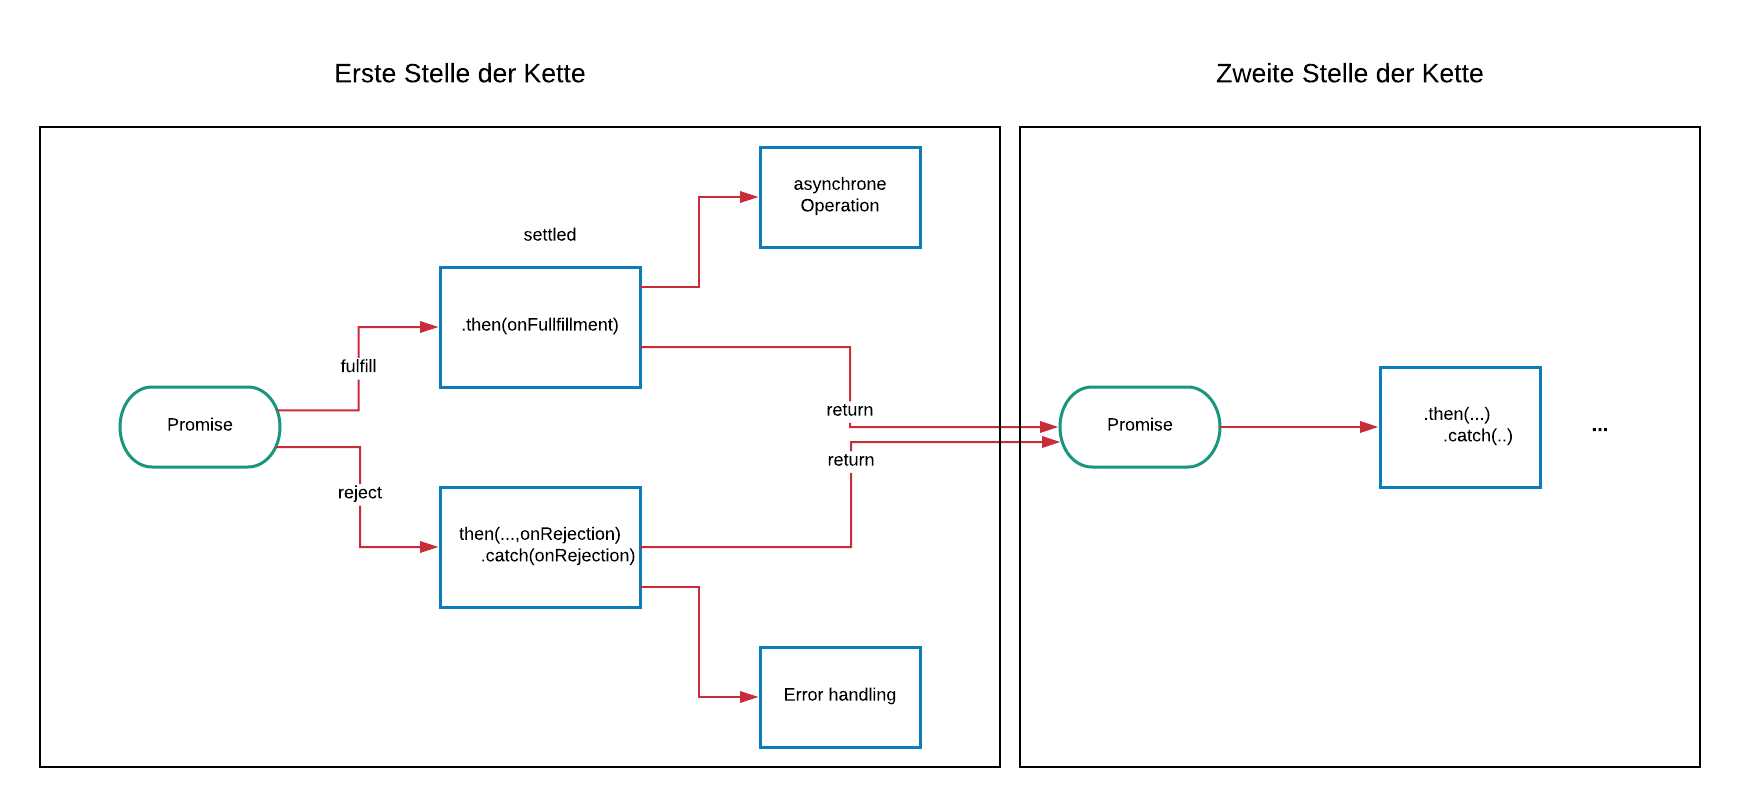
\includegraphics[width=13cm]{Promises-workflow}
\caption{Weiterreichung eines Promise-Objekts\cite{promise-executor}.}
\label{promise-chain-graphic}
\end{figure}

\noindent
Promise-Fehlschläge können dabei auf zwei verschiedene Wege gefangen werden. Innerhalb der then()-Methode kann eine zweite, optionale Funktion für das \textbf{Nicht-Eintreffen} der Operation festgelegt werden. In einem fiktiven Beispiel würde dies wie folgt aussehen:

\begin{figure}[H]
\begin{lstlisting}[basicstyle=\small]
get('story.json').then((response) => {
  console.log('Success!', response);
}, (error) => {
  console.log('Failed!', error);
})
\end{lstlisting}
\caption{Error-Handling innerhalb der then() Methode\cite{callback-vs-promises}.}
\end{figure}

\begin{figure}[H]
\begin{lstlisting}[basicstyle=\small]
get('story.json').then((response) => {
  console.log('Success!', response);
}).catch((error) => {
  console.log('Failed!', error);
})
\end{lstlisting}
\caption{Error-Handling mit der catch() Methode\cite{callback-vs-promises}.}
\label{error-with-catch}
\end{figure}

\noindent
Im Gegensatz zur oberen Variante führt die catch()-Methode keine zusätzlichen Operationen aus. Sie macht den Code lediglich semantisch lesbarer. Wichtig zu beachten ist, dass innerhalb einer Executor-Funktion \textbf{niemals} beide Argumente gemeinsam eintreffen können. Sie verhalten sich exklusiv. Deshalb ist das letztere Beispiel im Verhalten vergleichbar mit diesem:

\begin{figure}[H]
\begin{lstlisting}[basicstyle=\small]
get('story.json').then((response) => {
  console.log('Success!', response);
}).then(undefined, (error) => {
  console.log('Failed!', error);
})
\end{lstlisting}
\caption{Verhält sich ähnlich wie in Abbildung \ref{error-with-catch}.}
\end{figure}

\noindent
Der Unterschied ist minimal, aber extrem hilfreich. Promise-Fehlschläge gelangen bei der nächsten then() Methode in den fehlgeschlagen Callback weiter oder in die catch Methode(,wenn vorhanden). Mit then(func1, func2) wird entweder die erste oder die zweite Funktion aufgerufen, aber niemals beide. Jedoch mit then(func1).catch(func2) werden beide Callbacks aufgerufen, sollte die erste Funktion fehlschlagen. Dies ist nur Möglich, da die Funktionen in unterschiedlichen Stellen der Verkettung liegen. Neben den Prototyp-Methoden gibt es, wie bereits erwähnt, die statischen Methoden. Die wichtigsten dabei sind:

\begin{description}

\begin{figure}[H]
\item \begin{lstlisting}[basicstyle=\small]
Promise.race(iterable)
\end{lstlisting}

\item \begin{lstlisting}[basicstyle=\small]
Promise.all(iterable)
\end{lstlisting}
\caption{Ein iterable ist alles was mit einer for-of Schleife (ab ES6 nutzbar) iterierbar ist. Beispielsweise: Arrays oder Strings.}
\end{figure}
\end{description}

\noindent
Diese Methoden helfen Promises leichter zu verarbeiten. Beispielsweise, wenn es darum geht mehrere Promises voneinander abhängig auszuführen, hat man entweder die Wahl die Promise-Verkettung zu nutzen oder die Promises in einem Array zu lagern und dann die nötigen Aktionen mit der Sammlung von Promises auszuführen. Im nächsten Beispiel wird die \textbf{Promise-Verkettung}, \textbf{Promise.all()} und \textbf{Promise.race()} gegenübergestellt.

\begin{figure}[H]
\begin{lstlisting}[basicstyle=\small]
module.exports = {
    mode: 'development',
    entry: './src/modules/promises/stories-usage.ts',
    ...
}
\end{lstlisting}
\caption{Zum Ausführen der Beispiele muss ../promises/stories-usage.ts als Eingangsdatei konfiguriert werden.}
\end{figure}

\begin{figure}[H]
\begin{lstlisting}[basicstyle=\small]
export class HTTP {

    public makeRequest(url: string): Promise<any> {
        return fetch(url).then(response =>
            this.fakeLatency().then(() =>
                response.json()));

    }

    private fakeLatency() {
        return new Promise((resolve) =>
            setTimeout(resolve, 3000 * Math.random()));
    }
}

export class Story {

    public static BASE_URL = 'https://jsonplace.../posts/';
    public spinnerElement: HTMLElement;

    public http: HTTP = new HTTP();

    constructor() {
       this.spinnerElement = Story.createElm('<svg>..</svg>');
    }

    public static createElm(innerHTML: string): HTMLElement {
        const div = document.createElement('div');
        div.innerHTML = innerHTML;
        document.body.appendChild(div);
        return div;
    }
    
    public getAllStories(): Promise<string> {
        return this.http.makeRequest(Story.BASE_URL);
    }

    public getChapter(chapter: number): Promise<string> {
        return this.http.makeRequest(Story.BASE_URL + chapter.toString());
    }
\end{lstlisting}
\end{figure}

\begin{figure}[H]
\begin{lstlisting}[basicstyle=\small]
    public spawn(content): void {
        if (content instanceof Array === false) {
            content = [content];
        }
        content.forEach(elm => {
            const snippet = document.createElement('div');
            snippet.innerHTML = '<h1>${elm.title}</h1>
                                 <div>
                                     <i>${elm.id}</i>
                                 </div>
                                 <p>${elm.body}.</p>';

            document.body.insertBefore(snippet, this.spinnerElement);
        });

    }
    
    public displayFinished(): void {
        this.spinnerElement.style.display = 'none';
        Story.createElement('All done!');
    }
}

const story = new Story();
\end{lstlisting}
\caption{Der Vorteil der Objektorientierung in diesem Fall ist die Kapselung der Logik in: Endpunkt-Aufruf anbieten und Endpunkt-Aufruf verarbeiten.}
\end{figure}

\noindent
Ähnlich wie im Beispiel des Callback-Kapitels wird von der REST-API JSONPlaceholder Kapitel in die DOM geladen. In diesem Fall wurde hingegen das objektorientierte Paradigma gewählt. Die Klasse HTTP macht mit makeRequest() eine Http-Anfrage gegen einen übergebenen Endpunkt. Die \textbf{Fetch API} stellt ein Javascript Interface zur Verfügung, um Ressourcen zwischen dem Netzwerk anzufragen. Im Gegensatz zur bisher genutzten Klasse \textbf{XMLHttpRequest}, gibt fetch() ein Promise Objekt zurück. Mit der Story Klasse wird der Endpunkt der Datenabfrage als Klassenvariable definiert. Darüberhinaus werden mit getAllStories() und getChapter() die Methoden für die Abfrage definiert. Sollte ein Anwendungsfall sein, alle Kapitel anzuzeigen, würde der Code mit Promises so aussehen:

\begin{figure}[H]
\begin{lstlisting}[basicstyle=\small]
story.getAllStories()
    .then((response) =>
        story.spawn(response)
    )
    .finally(() =>
        story.displayFinished()
    );
\end{lstlisting}
\end{figure}

\noindent
Alle Kapitel werden mit einem Aufruf am Endpunkt angefragt. Ist das Promise in den settled Zustand angelangt, werden die Kapitel im Browser abgebildet. Als letzte Stelle der Kette wird mit finally der Lade-Icon ausgeblendet und eine Nachricht angezeigt, dass alle Stories abgebildet wurden. Sollte jedoch ein Anwendungsfall sein, dass nur drei Stories im Browser angezeigt werden sollen, könnte das wie folgt aussehen: 

\begin{figure}[H]
\begin{lstlisting}[basicstyle=\small]
console.time('Promise-Verkettung');
story.getChapter(1) // (*)
    .then((response1) => story.spawn(response1))
    .then(() => story.getChapter(2)) // (**)
    .then((response2) => story.spawn(response2))
    .then(() => story.getChapter(3)) // (***)
    .then((response3) => story.spawn(response3))
    .finally(() => {
        story.displayFinished();
        console.timeEnd('Promise-Verkettung');
    });
\end{lstlisting}
\caption{Promise-Verkettung für sequentielle Ausführungen}
\label{Promises-sequential-calls}
\end{figure}

\noindent
In diesem Fall werden nacheinander drei Kapitel angefragt und im Browser angezeigt. Da die Aufrufe im verketteten Konstrukt voneinander abhängig sind, addiert sich die Zeit die gebraucht wird, um ein Kapitel anzufragen und abzubilden. Die Idee dahinter ist, dass nach jedem Kapitelaufruf und -anzeige gewartet wird, bis dieser Vorgang abgeschlossen ist. Der Fluss sieht dabei so aus:

\begin{enumerate}
    \item Das erste Promise getChapter(1) wird aufgerufen(*). Der Status dieses Promise ist erstmal im pending Zustand.
    \item Bei Ankunft der Antwort, gelangt getChapter(1) in den settled Zustand. Die Daten \textit{response1} werden mit spawn(\textit{response1}) in einer neuen Stelle der Kette in die DOM geladen.
    \item Das nächste Promise getChapter(2) wird aufgerufen(**). Der Status dieses Promise ist erstmal im pending Zustand. 
    \item Bei Ankunft der Antwort, gelangt getChapter(2) in den settled Zustand. Die Daten \textit{response2} werden mit spawn(\textit{response2}) in einer neuen Stelle der Kette in die DOM geladen.
    \item ...
\end{enumerate}

\begin{figure}[H]
\centering
\includegraphics[width=12cm]{Promise-Verkettung-Stories.png}
\end{figure}

\noindent
Dieser Vorgang endet mit der finally() Verarbeitungsmethode. Zu beachten ist, dass das gesamte verkettete Konstrukt in einem eigenen Thread läuft. Innerhalb dieses Threads verlaufen die Operationen sequentiell. Das liegt daran, da die jeweilige then() Methode ein Promise-Objekt weiterreicht. Somit kann das nächste then() entsprechend nach entstandenem Status und Wert weiterarbeiten. Obwohl die Aufrufe in der Darstellung deutlich lesbarer als ineinandergeschachtelte Callbacks sind, wird mit diesem Beispiel ebenfalls deutlich, dass bei Promise-Verkettungen der Code nun aneinandergeschachtelt ist. Es ist immer noch zur erkennen, dass Operationen nicht innerhalb des synchronen Flusses verarbeitet werden. Die nächste Variante ist, die Kapitel in einem Promise Array zu lagern und parallel mit Promise.all() auszuführen.

\begin{figure}[H]
\begin{lstlisting}[basicstyle=\small]
const chapters: Array<Promise<void>> = [];

for (const n of [1, 2, 3]) {
    chapters.push(story.getChapter(n));
}

console.time('Promise-all');
Promise.all(chapters).then((response) =>
    story.spawn(response)
).finally(() => {
    story.displayFinished();
    console.timeEnd('Promise-all');
});
\end{lstlisting}
\caption{Promise.all(iterable) bekommt ein iterierbares Objekt als Parameter übergeben}
\label{Promise-all-example}
\end{figure}

\noindent
Ein Promise.all() kann dabei abhängig vom Übergabeparameter verschiedene Rückgabewerte haben. Sollte das eingegebene iterable Argument leer sein, wird Promise.all() synchron erfüllt. Wenn das eingegebene iterable Argument keine Promises enthält, kommt ein asynchron eingelöstes Promise heraus. In allen anderen Fällen gibt ein Promise.all() ein einzelnes ausstehendes Promise zurück, dass eintrifft wenn alle Promises innerhalb des übergebenen Promise-Arrays eingetroffen sind. Die Rückgabewerte entsprechen dann der Reihenfolge der Promises in dem Array, unabhängig von der Reihenfolge des Erfüllungszeitpunkts \cite{promise-all}. Sollte ein Promise fehlschlagen, wird promise.all() ebenfalls fehlschlagen mit der Fehlernachricht des ersten fehlgeschlagenen Promises \cite{promise-executor}.\\

\begin{figure}[H]
\begin{lstlisting}
Promise-all: 1974.587890625ms
Promise-Verkettung: 4905.918701171875ms
\end{lstlisting}
\caption{Vergleich der Gesamtausführungszeit.}
\label{comparison-promise-all-and-chained-promise}
\end{figure}

\noindent
Dabei ist zu beachten, dass die Promises parallel voneinander ausgeführt werden. Der unterschied der verketteten Variante zu Promise.all() liegt in der Art und Weise der Ausführung. Ein Promise.all() führt die Promises parallel aus und löst sich nur so schnell auf wie das langsamste eintreffende Promise im iterable. Solange passiert nichts. In diesem Fall wird solange wird kein Kapitel in die DOM geladen, bis das langsamste Kapitel eingetroffen ist. Dafür ist aufgrund der parallelen Ausführung die Gesamtladezeit mit Promise.all() schneller (siehe Abb. \ref{comparison-promise-all-and-chained-promise}). In der verketteten Variante hingegen werden die Kapitel nacheinander verarbeitet. Der Nutzer bekommt den sequentiellen Ladevorgang der Kapitel mit. In der Praxis sollte genau abgewogen werden, welches Umsetzungskonzept in welcher Situation mehr Sinn macht.

\begin{figure}[H]
\centering
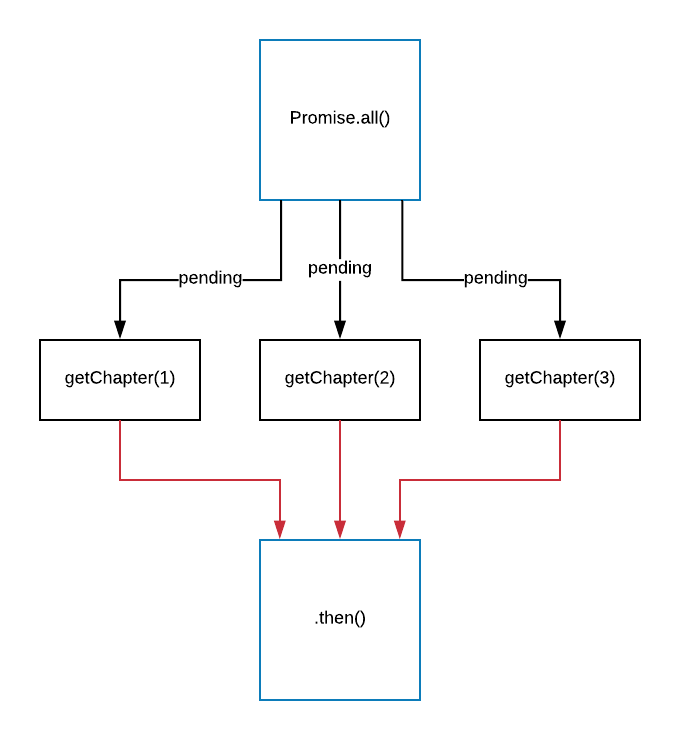
\includegraphics[width=7cm]{promise-all}
\caption{Die Nachrichten werden in der Reihenfolge ausgegeben, in der sie ins Array übergeben worden sind.}
\end{figure}

\noindent
Dagegen wird die nächste Methode verhältnismäßig seltener genutzt. Promise.race(iterable) gibt ein erfolgreiches oder fehlgeschlagenes Promise zurück, sobald eines der Promises in dem iterable erfolgreich war oder fehlgeschlagen ist, entsprechend mit dem Wert dieses Promises. Wenn das übergebene iterable leer ist, wird das Promise für immer im pending Status verharren\cite{promise-race}.

\begin{figure}[H]
\begin{lstlisting}[basicstyle=\small]
Promise.race(chapters).then((response) =>
    story.spawn(response)
).finally(() =>
    story.displayFinished()
);
\end{lstlisting}
\caption{Es wird schnellste ladende Kapitel angezeigt.}
\end{figure}

\subsection{Anti-Patterns und Best Practices}

Ob bei der Erstellung oder bei der Verarbeitung von Promises - es gibt gewisse Ansätze nach denen man sich bei der Nutzung richten sollte. Ein negativ Beispiel für die Verarbeitung von Promises, wäre folgendes:

\begin{figure}[H]
\begin{lstlisting}[basicstyle=\small]
story.getChapter(1)
    .then((response1) => {
        story.spawn(response1);
        story.getChapter(2)
            .then((response2) => {
                story.spawn(response2);
                story.getChapter(3).then((response3) =>
                    story.spawn(response3)
                ).finally(() => 
                    story.displayFinished()
                    );
            });
    });
\end{lstlisting}
\caption{Schachtelung nach dem Callback Muster.}
\end{figure}

\noindent
Diese Methoden rufen ähnlich wie in Abbildung \ref{Promises-sequential-calls} drei Kapitel nacheinander auf. Obwohl sie im positiv Fall der API-Aufrufe die Kapitel sequentiell laden, wird hier komplett auf den Vorteil, den Promises gegenüber Callbacks bieten, verzichtet. Zudem ist die gesamte Kette davon abhängig, ob der erste Promise-Aufruf eintrifft. Hier wird keinerlei Möglichkeit gewährleistet ein Fehlschlag des ersten Aufrufs zu fangen ohne Code-Duplizierung. Solche ineinandergegliederte Promise-Verschachtelungen werden unter Entwicklern auch als \glqq{}Promise-Hell\grqq{} bezeichnet.
Mit dem ursprünglichen Beispiel von Abb. \ref{Promises-sequential-calls} ist es jedoch Möglich Fehler zwischen der Kette zu fangen:

\begin{figure}[H]
\begin{lstlisting}[basicstyle=\small]
story.getChapter(1)
    .then(() => {
        throw new Error('Faked Error');
    })
    .catch((err) => {
        console.log(err);
        return story.getChapter(2);
    })
    .then((response2) => story.spawn(response2))
    .then(() => story.getChapter(3))
    .then(response3 => story.spawn(response3))
    .finally(() => story.displayFinished());
\end{lstlisting}
\caption{Das erste Kapitel wird nicht abgebildet, jedoch alle folgenden.}
\end{figure}

\noindent
Als Faustregel für Promises sollte beachtet werden, dass sie nur für einmalig auftretende asynchrone Events genutzt werden sollten. Der Verarbeitungsstatus eines Promise kann folgend sein:

\begin{description} 
\item Pending: Der Ausgang des Promises ist noch ungewiss.
\item Resolved: Die Aktion, die zum Promise verlief, ist eingetroffen.
\item Rejected: Die Aktion, die zum Promise verlief, schlug fehl.
\item Settled: Die Aktion ist entweder fehlgeschlagen oder eingetroffen - jedoch abgeschlossen.
\end{description}

\noindent
Beim erstellen einer Promise Instanz werden zwei Callback Funktionen als Argument angenommen. Resolve() wird mit der then() Methode verarbeitet und reject() mit der catch() Methode gefangen. Finally() kann unabhängig vom Eintreffen oder Fehlschlagen einer Operation genutzt werden. Der zurückgegebene Typ einer Promise Methode ist immer ein Promise-Objekt. Aufgrund dessen lassen sich Promises leicht verketten. Promises bieten mit Promise.all() und Promise.race() Hilfemethoden an, um mehrere Promises leichter zu verarbeiten.




